The final section of the thesis is concerned with trying to constrain the mass of protoplanets embedded in disks by quantitatively extracting the planet wake from kinematic observations.
We will build on the work presented in \citet{calcino2022}, where we showed that one can trace the shape of the planet wake, and amplitude of velocity kinks, through the peak velocity map.
In Section~\ref{sec:v0_fitting} we attempt to create a planet mass fitting procedure using synthetic peak velocity maps generated by projecting \textsc{wakeflow} models to the emitting surface of the disk.
Additionally, in Section~\ref{sec:mirror_residuals}, we present a method for locating the wake such as that in \citet{calcino2022}, but that does not rely on identifying patterns by eye.
%Finally in Section~\ref{sec:isovelocity_transform}, we demonstrate a potential method for extracting the wake information from observations that is model-independent.

\section{Peak velocity fitting} \label{sec:v0_fitting}

As shown in \citet{calcino2022}, the planet wake manifests in the peak velocity ($v_0$) map generated from molecular line emission observations as spatially correlated deviations from the expected smooth iso-velocity contour.
We additionally created synthetic $v_0$ maps by projecting semi-analytic models of the planet wake plus background rotation (Equation~\eqref{eq:rot_eq_full}) to a the emitting layer of the disk, and then calculating the line-of-sight velocities in the disk.
Here, we will take the same approach to generating $v_0$ maps, but we will fit them onto the observed peak velocities.
The advantage of fitting in this way instead of first subtracting a best-fitting model for the background rotation and fitting to the residuals is two-fold.
First, creating residuals in this way is known to easily confuse the sign of the perturbations due to the high sensitivity to the background model (see the Appendix of \citealt{calcino2022}).
Secondly, fitting simultaneously for the background instead of assuming it allows for the determination of the covariances in the uncertainties between the background and planet perturbation models.
The best-fitting parameters for the planet mass and location will therefore not be conditioned on some background model, and we will be able to see any potential degeneracies between the parameters of each model.

\subsection{Models}

To generate our models, we first calculate the height of the emitting layer in the disk using the parameterisation \citep{pinte2018}
\begin{align}
    z(r) = z_0 \left( \frac{r}{r_{\rm ref}} \right)^\phi \exp \left( -\left[ \frac{r}{r_\mathrm{taper}} \right]^{\psi} \right), \label{eq:height}
\end{align}
which gives a flared structure with an exponential taper. $z_0$, $\phi$, $r_{\rm taper}$ and $\phi$ are then all model parameters that determine the height of the emitting layer. 
$r_{\rm ref}$ simply determines the radius at which the reference height $z_0$ and other parameters are defined, and we just set it to 100 au.
While this is a lot of freedom, the idea is to eventually use other methods of determining the height in this form such as the code \textsc{dynamite}\footnote{\url{https://github.com/cpinte/dynamite}} \citep{pinte2018} to determine best-fitting parameters, and then to place strong priors on the same parameters when fitting for the planet mass.

We then calculate the background velocity $v_{\phi,\mathrm{0}}$ for the disk at this emitting layer on a $300 \times 300$ Cartesian grid using
\begin{align}
    v_{\phi,\mathrm{0}}(r,z) = \sqrt{\frac{G M_\star}{r}} \left[ - \left(p + 2q\right) \left( \frac{H}{r} \right)^2 + \left( 1-2q \right) + \frac{2qr}{\sqrt{r^2 + z^2}}\right]^{1/2}, \label{eq:omega_wf_ps_full}
\end{align}
which is just Equation~\eqref{eq:omega_wf_ps} rewritten as a velocity.
$p$ and $q$ determine the amount of pressure support in the disk, where $\rho \propto r^{-p}$ and $c \propto r^{-q}$ as usual.
$M_\star$ is the mass of the central star.
The scale height $H$ is calculated using
\begin{align}
    H(r) = H_{\rm ref} \left( \frac{r}{r_{\rm ref}} \right)^{\frac{3}{2} - q},
\end{align}
which comes from Equation~\eqref{eq:scale_height}.
Thus $q$, $p$, $H_{\rm ref}$ and $M_\star$ are model parameters that determine the background rotation of the disk.

Next, the planet perturbations are calculated by calling \textsc{wakeflow} using the aforementioned parameters, as well as the planet mass $M_{\rm p}$ and orbital radius $r_{\rm p}.$
The calculated azimuthal velocity perturbations $v_{\phi,\mathrm{p}}$ and radial velocity perturbations $v_{r,\mathrm{p}}$ are then used with the background rotation $v_{\phi,\mathrm{p}}$ to calculate the total velocity components $v_r$ and $v_\phi$
\begin{align}
    v_r = v_{r,\mathrm{p}}, \qquad v_\phi = v_{\phi,\mathrm{0}} + v_{\phi,\mathrm{p}}.
\end{align}
These are then mapped to Cartesian components $v_x$ and $v_y$ so that we may use rotation matrices to obtain the line-of-sight velocities 
\begin{align}
    v_x &= -v_\phi \sin \phi + v_r \cos \phi, \\
    v_y &= +v_\phi \cos \phi + v_r \sin \phi.
\end{align}
Defining the velocity field in the frame of the disk $\mathbf{v} = (v_x, v_y, v_z)$ where we set $v_z=0$, we find that the velocity field projected to the sky plane $\mathbf{v'}=(v_x', v_y', v_z')$ is given by 
\begin{align}
    \mathbf{v'} =  R_z(p) R_x(i) R_z(\phi_{\rm p}) \, \mathbf{v}
\end{align}
where $R_x$ and $R_z$ are the standard Cartesian rotation matrices around the $x$ and $z$ axis respectively, $p$ is the position angle of the disk on the sky, $i$ is the inclination of the disk, and $\phi_{\rm p}$ is the azimuthal position of the disk as measured in plane of the disk.
The line-of-sight velocity is then simply given by the $v_z'$ component of the above.
Likewise, we can find the positions associated with the velocity field by rotating the position scalar field $\mathbf{x} = (x,y,z)$ in the same way to find $\mathbf{x'} = (x',y',z')$.
The sky coordinates $\Delta \, \mathrm{RA}$ and $\Delta \, \mathrm{Dec}$ in arcseconds for our projected line-of-sight velocity field is then simply
\begin{align}
    (\Delta \, \mathrm{RA}, \Delta \,\mathrm{Dec}) = \frac{1}{D} (x', y'),
\end{align}
where $D$ is the distance to the source in parsecs.

Figure~\ref{fig:model_v0} shows an example peak velocity map generated using this method for the disk of HD~163296, using the parameters from \citet{calcino2022} but with a planet mass of $1 \, \mathrm{M_J}$.

\begin{figure}
    \centering
    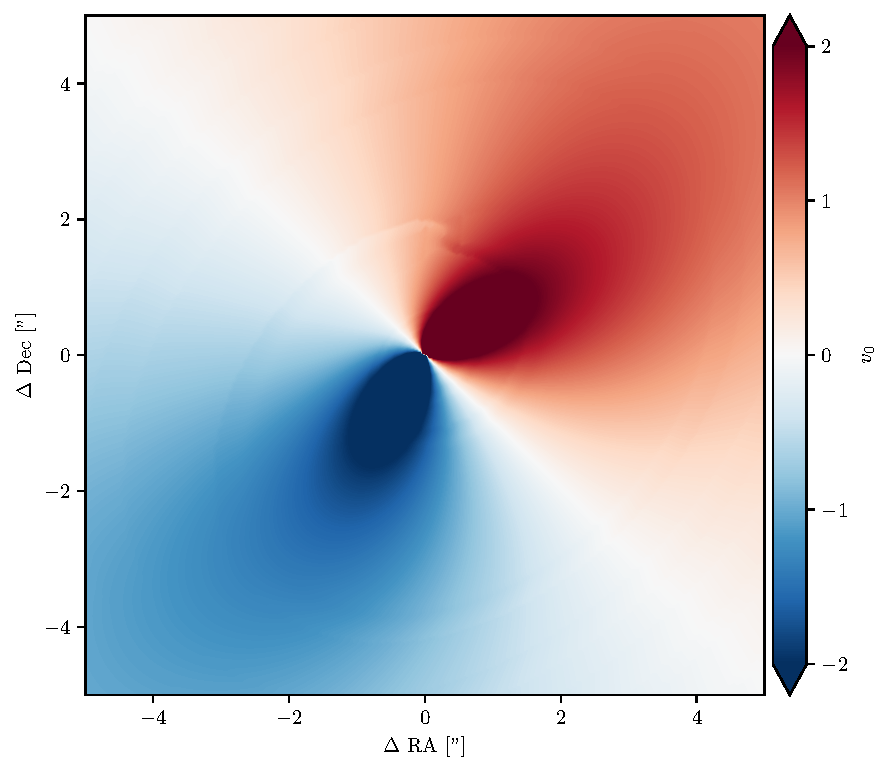
\includegraphics[width = 0.7\textwidth]{figures/thesis_contours_obs_model.pdf}
    \caption{Synthetic peak velocity map generated by projecting a semi-analytic model to the emitting layer. Parameters used in the model taken from \citet{calcino2022}, except for the planet mass which was set to $1 \, \mathrm{M_J}$. The planet wake is visible in the map due to the velocity perturbations it causes. The wake is most visible along near the semi-major axis as expected for radial-dominated motion \citep{rafikov2002a,bollati2021a,calcino2022}.}
    \label{fig:model_v0}
\end{figure}

\subsection{Fitting procedure}

Peak velocity maps produced from real kinematic observations are discretised in velocity at a resolution equal to the spacing of the channels\footnote{Unless using the higher order quadratic method mentioned in Section~\ref{sec:obs_analysis_garg}. Here we choose to use the usual peak velocity so that our uncertainties are related only to the beam size of the observations, and thus the positions of the iso-velocity contours. Using the quadratic method introduces statistical uncertainties in the velocities themselves.}.
We therefore discretise the velocity field from our models using the channel spacing.
Since the planet induces wiggles in the iso-velocity curves, we performed the fitting by minimising the distance between corresponding curves from the model and observations.
In a peak velocity map, we can find these curves simply through making a contour plot.
We therefore extracted the iso-velocity curves from both the observations and models by creating a contour plot with the \textsc{Python} package \textsc{Matplotlib}, which calculates the points along the contours using a marching squares algorithm \citep{hunter2007}.
Since peak velocity maps calculated from observations tend to be noisy, and often suffer from contamination by the lower surface of the disk, the calculated contours may be discontinuous towards the edge of the disk.
We therefore take only the longest continuous contour returned as representative of the iso-velocity curve for a specific velocity, and discard the others.
This can be seen in the left panel of Figure~\ref{fig:conts_obs_model}, which shows the peak velocity map from MAPS $^{12}$CO observations \citep{oberg2021} that we used in \citet{calcino2022}.
In the top left of the panel, we can see many small blobs due to backside contamination.
They grey lines show the contours that we extract, and the blobs are ignored.
The middle panel of Figure~~\ref{fig:conts_obs_model} shows the equivalent iso-velocity curves extracted from our example model in the previous section, this time without an embedded planet.
The right panel overlays the extracted model contours with the peak velocity map from the left panel.

\begin{figure}
    \centering
    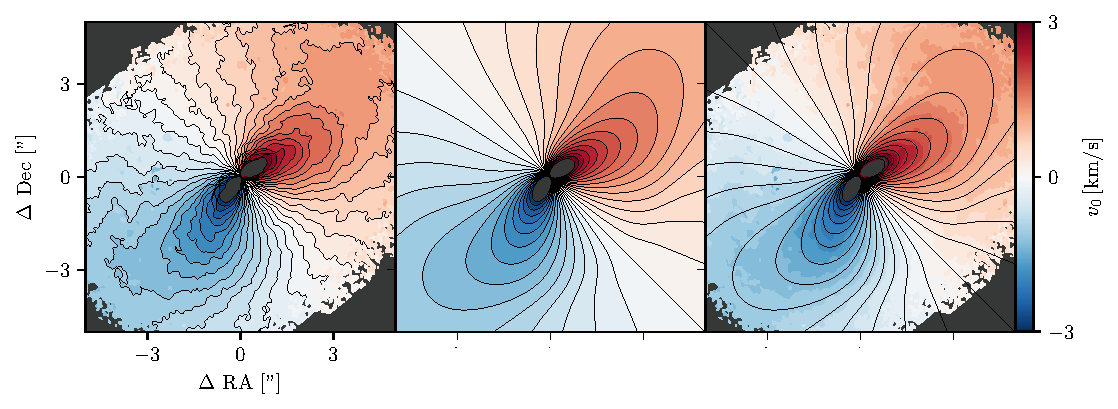
\includegraphics[width = 0.99\textwidth]{figures/thesis_plot_model_obs.pdf}
    \caption{The left panel shows a plot of the peak velocity map calculated from the $0.15"$ resolution $^{12}$CO line emission observations of the circumstellar disk of HD~163296 \citep{oberg2021}, with the contours extracted by our algorithm plotted in grey. The middle panel shows our model, with the extracted contours again plotted in grey. The right panel shows the contours extracted from the model plotted over the observed peak velocity.}
    \label{fig:conts_obs_model}
\end{figure}

In order to perform the fitting, we need some notion of distance between the lines of iso-velocity in the model and observations.
To do this, we summed the Euclidean distance between nearest points along each contour.
That is, for each point $(x_{\mathrm{o},j},y_{\mathrm{m},j})$ along for example the $\Delta v = 200 \, \mathrm{m/s}$ iso-velocity curve in the observations, we found the closest point $(x_{\mathrm{m},j},y_{\mathrm{m},j})$ on the $\Delta v = -200 \, \mathrm{m/s}$ iso-velocity curve in the model, and calculated the distance $d_j^2 = (x_{\mathrm{o},j} - x_{\mathrm{m},j})^2 + (y_{\mathrm{o},j} - y_{\mathrm{m},j})^2$.
Summing these distances then yields the total ``distance'' between the two curves $D = \sum_j d_j$.
This distance was calculated for all of the pairs of iso-velocity curves extracted.
The uncertainty in this distance is $\sigma_{\rm beam}$, which is the angular size of the telescope resolution.
We therefore chose our reduced chi squared to be
\begin{align}
    \chi_{\rm red}^2 = \left( \sum_i^{N_{\rm C}} N_i - N_{\rm p} \right)^{-1} \left( \sum_{i}^{N_{\rm C}} \sum_{j}^{N_i} \frac{(x_{\mathrm{o},ij} - x_{\mathrm{m},ij})^2 + (y_{\mathrm{o},ij} - y_{\mathrm{m},ij})^2}{\sigma_{\rm beam}^2} \right),
\end{align}
where the $i$ index sums over each iso-velocity contour of a particular line-of-sight velocity, and the $j$ index sums over all the points along that contour.
$N_i$ is therefore the number of points along observed contour $i$, while $N_{\rm C}$ is the total number of contours.
$N_{\rm p}$ is the number of parameters in the model.

\subsection{Background fitting}

Before attempting to fit for planet mass, we wanted to confirm that we could obtain $\chi^2$ minima in parameter space for sensible values of a model including only the unperturbed background disk.
To do this we used the JvM corrected \citep{jorsater1995} $^{12}$CO $J=2-1$ \textit{robust=0.5} line emission observations of HD~163296 from the MAPS large program (2018.1.01055.L, \citealt{oberg2021,czekala2021})\footnote{The data are available for download at \url{http://alma-maps.info/}.}, which has a channel spacing of $200 \mathrm{m/s}$, and a beam size of $0.15"$.
This is the same data we used in \citet{calcino2022}.
We also assumed a systemic velocity of $v_{\textrm{los}}= 5.76$ km/s \citep{teague2021} and a distance of $101.5 \, \mathrm{pc}$ \citep{gaiacollaboration2018}.

We then adopted the best-fitting background model parameters used in \citep{calcino2022}, and varied only parameter one at a time to see whether each found a minimum $\chi^2$ value.
The results of the grid search are shown in Figure~\ref{fig:grid_chisq_background}.
The top row of the figure shows the parameters that determine the background rotation.
We see that for the rotation parameters, both $M_\star$ and $H_{\rm ref}/r$ find minima around approximately $1.8 \, \mathrm{M_\star}$ and $0.11$ respectively. 
These both compatible with the expected values from the literature, differing by less than 5\% in each case \citep{pinte2018a}.
However the $p$ and $q$ indices are both constrained very poorly and neither find a minimum.
This is perhaps not surprising when considering that changing either of this has little effect on our model, as they merely change the background rotation very slightly as part of the pressure gradient term.
The aspect ratio $H/r$ is also only responsible for the pressure correction, but since it is squared in Equation~\eqref{eq:omega_wf_ps_full} it has a larger effect.
It therefore seems unlikely that $p$, $q$ and $H/r$ could be disentangled from fitting purely our background model.
However, both $H/r$ and $q$ are both responsible for determining the shape of the wake once we add a planet (see Equation~\ref{eq:power_law_wake}), which may allow us to constrain them more effectively.

\begin{figure}
    \centering
    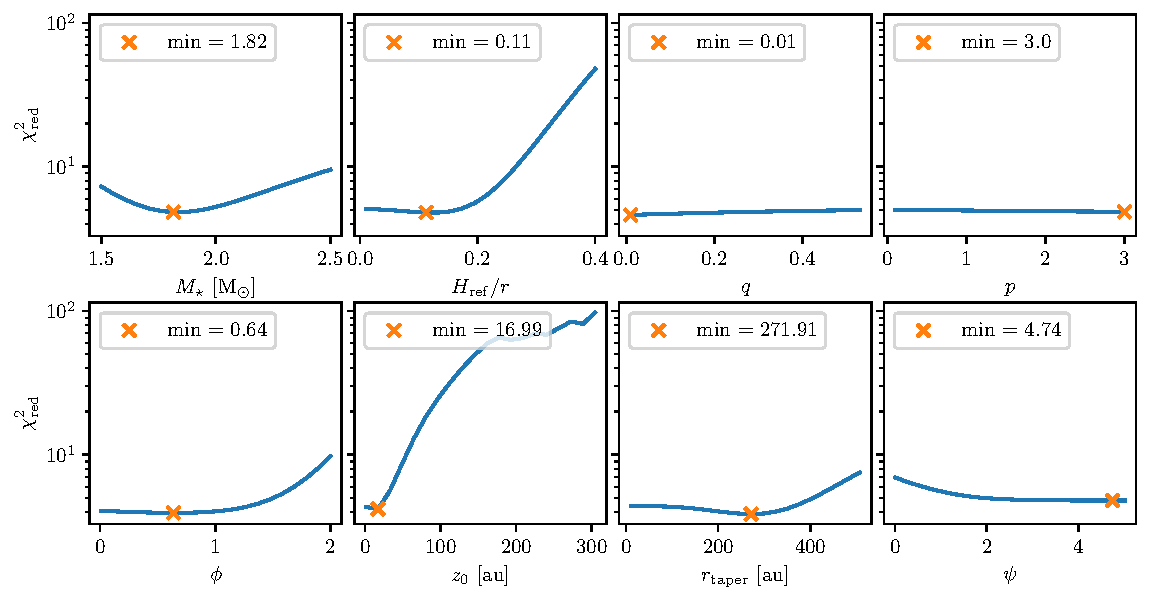
\includegraphics[width = 0.95\textwidth]{figures/chi_sq_background_hd163.pdf}
    \caption{$\chi_{\rm red}^2$ values fitting an unperturbed disk model to the MAPS $^{12}$CO peak velocity map of the HD~163296 disk, calculated by varying each parameter one at a time while keeping the others fixed. The top row is parameters tha determine the disk rotation, while the bottom row parameters determine the $^{12}$CO emission surface. The parameter values for the best-fit are marked by orange crosses. We see that the parameters that determine the pressure support $p$ and $q$, as well as the disk taper rate $\psi$, are poorly constrained.}
    \label{fig:grid_chisq_background}
\end{figure}

Turning our attention to the parameters that determine the emission surface, shown in the bottom row of Figure~\ref{fig:grid_chisq_background}, we see that all the parameters found a minimum.
These minima occur at values of $\phi = 0.64$, $z_0 = 16.99 \, \mathrm{au}$, $r_{\rm taper} = 271.91 \, \mathrm{au}$, and $\psi = 4.74$.
Comparing with the values found by \citet{law2021a}, which were $\phi = 1.851$, $z_0 = 39.37 \, \mathrm{au}$, $r_{\rm taper} = 239.74 \, \mathrm{au}$, and $\psi = 1.182$, we see that $\phi$, $z_0$ and $\psi$ are significantly different.
The difference in $\psi$ is not too surprising, as the rate of exponential taper of the height of the disk likely does not effect the model very much.
This is because the taper really only starts to have an effect at around $300$ au or $\sim3"$, which is near the edge of the data.
The cause of the difference in values were obtained for $\phi$ and $z_0$ is less clear.
They imply that the inner disk stays flatter for longer than found by \citet{law2021a}, before rising more steeply in the outer disk.
This may be due to our method of calculating $\chi^2$, which relies on Euclidean distances.
Changing the height in the inner disk does not result in much change to the iso-velocity contours, and so measuring the height in the inner disk in this way perhaps provides a poor constraint.
The results do seem to recover the height in the outer disk more accurately, since $r_{\rm taper}$ is relatively close to the \citet{law2021a} value.
Of course, all this comes with the important caveat that each minimum is conditioned on the other parameters being correct, since we are varying them one at a time here.

\subsection{Planet fitting}

Next, we performed the same analysis as above, except including the perturbations induced by a planet.
We used a $2.0 \, \mathrm{M_J}$ planet, placed at an orbital radius of $256$ au and a planet azimuth of $55$ degrees \citep{pinte2018a,calcino2022}.
The results for the background parameters are presented in Figure~\ref{fig:grid_chisq_planet_bg}, while the results for the planet parameters are shown in Figure~\ref{fig:grid_chisq_planet}.

For the background parameters shown in the top row, all of the minima are different to those found in Figure~\ref{fig:grid_chisq_background}, where a planet was not included. The central star mass has increased by $\sim10$\%, $H_{\rm ref}/r$ has halved, and $p$ and $q$ show different behaviours.
There are multiple possible explanations for this.
The first, and more straightforward, is that the kinks we have added to the model contours by including a planet allows for a better fit to background features.
Alternatively, it may be due to the effect those parameters have on the planet perturbations.
For example, reducing $H_{\rm ref}/r$ will significantly reduce the value of the thermal mass (see Equation~\ref{eq:thermalmass}).
This in turn increases the value of $M_{\rm p} / M_{\rm th}$, resulting in larger kink amplitudes.
$H_{\rm ref}/r$ and $q$ both determine the shape of the wake (see Equation~\ref{eq:power_law_wake}), which is likely to change how well the kinks fit the data.

For the emission surface parameters (bottom row of Figure~\ref{fig:grid_chisq_planet_bg}), we again find differences to the purely background fit.
$\phi$ and $z_0$ are both larger, which in each case increases the height of the emitting layer\footnote{More precisely, increasing $\phi$ makes the emitting layer more flared, whereas increases $z_0$ scales the height by a constant for all $r$.}.
The radius of the taper is $\sim 25$\% larger, which has the result fo increasing the height of the disk model in the region around $300$ au.
The result for $\psi$ is not much different, with a similar behaviour to in the background case where any large value of $\psi$ performs well.
These differences in height corroborate the idea that adding the planet kinks can result in a different best-fit for just the background as already mentioned.
These parameters do not have any effect of the shape of the wake or the amplitude of the kinks, unlike the parameters that determine the rotation.

\begin{figure}
    \centering
    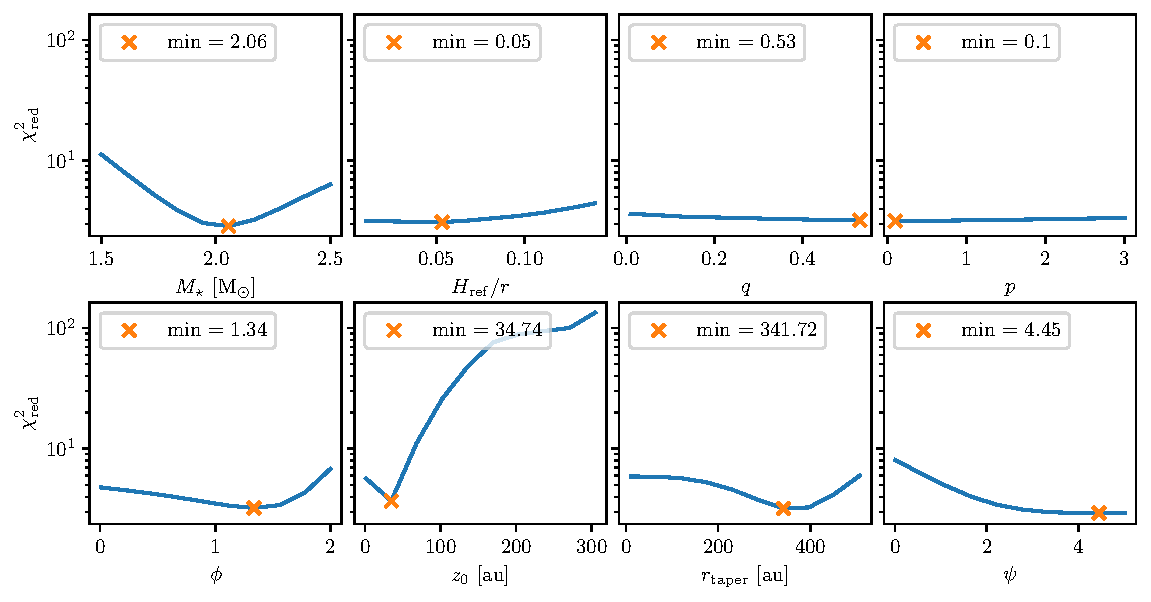
\includegraphics[width = 0.95\textwidth]{figures/chi_sq_background_planet_hd163.pdf}
    \caption{$\chi_{\rm red}^2$ values fitting an disk model with a $2 \, \mathrm{M_J}$ perturbing planet to the MAPS $^{12}$CO peak velocity map of the HD~163296 disk, calculated by varying each parameter one at a time while keeping the others fixed. The top row is parameters tha determine the disk rotation, while the bottom row parameters determine the $^{12}$CO emission surface. The parameter values for the best-fit are marked by orange crosses. The introduction of a planet results in different local minima for the background disk parameters.}
    \label{fig:grid_chisq_planet_bg}
\end{figure}

\begin{figure}
    \centering
    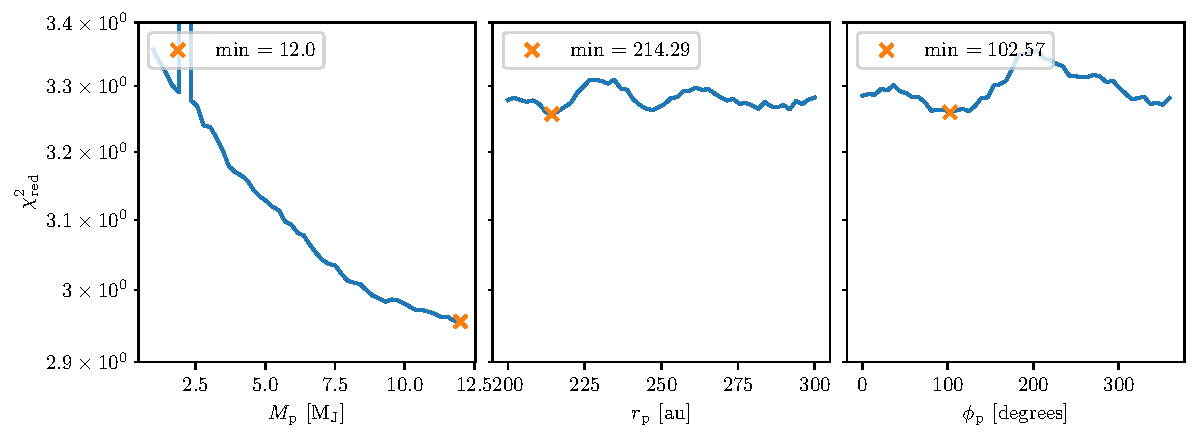
\includegraphics[width = 0.95\textwidth]{figures/chi_sq_planet_hd163.pdf}
    \caption{$\chi_{\rm red}^2$ values fitting an disk model with a $2 \, \mathrm{M_J}$ perturbing planet to the MAPS $^{12}$CO peak velocity map of the HD~163296 disk, calculated by varying each parameter one at a time while keeping the others fixed. The left panel shows the result of varying the planet mass, while the middle and right panels show the results for varying $r_{\rm p}$ and $\phi_{\rm p}$ respectively. The parameter values for the best-fit are marked by orange crosses.}
    \label{fig:grid_chisq_planet}
\end{figure}

Figure~\ref{fig:grid_chisq_planet} shows the results for the planet parameters themselves.
Looking first at the planet mass, we see that the best fitting mass is the largest in the interval that we tried, $12.5 \, \mathrm{M_J}$.
We did not allow for planets larger than this as the semi-analytic solution becomes very inaccurate and poorly behaved (see Section~\ref{sec:high_mass}).
This result is surprising, as it has previously been found that a planet of mass $3$--$4 \, \mathrm{M_J}$ accurately recreates the velocity kink induced nearby the planet.
Additionally, $r_{\rm}$ actually finds two minima, one at around $240$ au, which is close to what we would expect from \citet{calcino2022}.
The other minimum at $215$ is intriguing, as there have been claims of an additional planet closer to the star \citep{teague2018,pinte2020}.
It may be that this minimum results from the wake attempting to fit the arc feature mentioned in \citet{teague2021} and \citet{calcino2022} (see the opaque crosses in Figure~1 of the latter).
Finally, $\phi_{\rm p}$ finds a minimum at $\sim100$ degrees, which is significantly different to the $\phi_{\rm p}=55$ degrees that we used in \citet{calcino2022}.
Since tightly-wound spiral structure varies rapidly in $\phi$ as the radius changes slowly, it may be that this is because the value of $r_{\rm p}=256$ au we have chosen is not quite correct.

\subsection{Model-model fitting} \label{sec:model_model_fit}

It is not exactly clear how to interpret the results presented in the previous section.
While minima were found for most of the background disk parameters, $q$ and $p$ were both very poorly constrained.
Furthermore, the best-fitting parameters changed significantly once a planet was added.
Most importantly, we did not find a minimum at a particular planet mass, instead the performance just increased with $M_{\rm p}$.
This is of particular concern since this is the value we are most interested in constraining.

To attempt to understand what is going on, we generated a synthetic observation using our models, and then performed a grid search in $\chi^2_{\rm red}$.
For the synthetic observation, we set the distance, inclination and position angle to $100$ pc, $-225$ degrees, and $45$ degrees.
We then chose background model parameters of $M_\star = 2.0 \, \mathrm{M_\odot}$, $H_{\rm ref}/r = 0.1$, $q=0.35$, $p=2.25$, $\phi=1.5$, $\psi=3.5$, $z_0 = 30$ au and $r_{\rm taper} = 400$ au.
The planet parameters were chosen to be $r_{\rm p} = 300$ au, $M_{\rm p}= 0.8 \, \mathrm{M_J}$, and $\phi_{\rm p}=45$.
All of the parameters are similar to those found by \citet{pinte2018a} and \citet{calcino2022} for HD~163295, except that we deliberately chose a low mass planet to rule out any strange effects from the high-mass regime in the semi-analytic model.

We then performed a grid search in $M_{\rm p}$ and $\phi_{\rm p}$, where all other parameters were set to their true values.
We used 20 evenly spaced $M_{\rm p}$ values in the range $0.5$ -- $1.5 \, \mathrm{M_J}$, and 20 evenly spaced $\phi_{\rm p}$ values in the range $0$ -- $90$ degrees.
For $\sigma_{\rm beam}$, we simply kept the value of $0.15"$ from the observations, since it merely provides a constant offset.
The result is shown in Figure~\ref{fig:planet_grid_search}, where the heatmap shows the resultant $\chi^2_{\rm red}$ value for each set of $M_{\rm p}$ and $\phi_{\rm p}$ values, while the true value is marked by a red dot.
We see that once again the best-fit is provided by the largest $M_{\rm p}$, as well as $\phi_{\rm p}= 0^\circ$.
This was surprising as the minimum in $\chi^2_{\rm red}$ therefore occurs nowhere near the true values, even for the case where we have every other parameter exactly correct. 
\begin{figure}
    \centering
    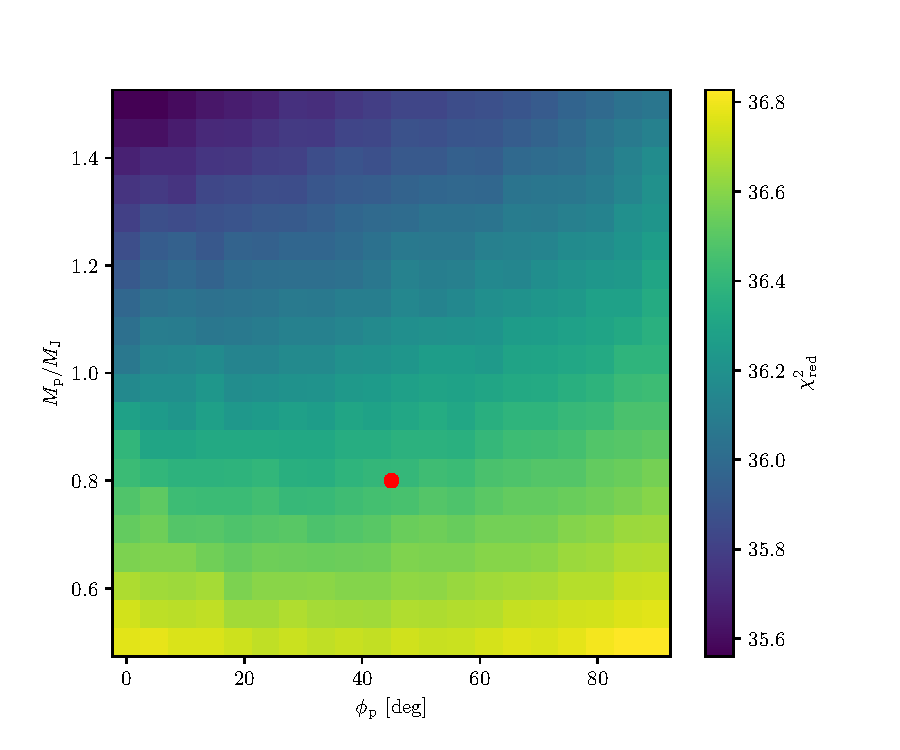
\includegraphics[width = 0.8\textwidth]{figures/planet_mass_az_grid_var.pdf}
    \caption{Grid search in $\chi^2_{\rm red}$ fitting synthetic observations generated with our model. $M_{\rm p}$ and $\phi_{\rm p}$ were both varied around their true values, while all other parameters were set exactly to the values used to generate the synthetic observations. We see that the minimum in $\chi^2_{\rm red}$ once again occurs for the highest mass planet provided, and is not centred on the true values shown by the red dot.}
    \label{fig:planet_grid_search}
\end{figure}

\subsection{Discussion}

The results obtained in Section~\ref{sec:model_model_fit} indicate that our choice of $\chi^2_{\rm red}$ is not well suited to the problem, as it does not find a minimum at the true value even in the case that the model matches the data exactly.
It is likely that this comes down to how the distance between the individual points are calculated.
Say for example we are finding the distance between contours $A$ and $B$.
For some point along $A$ we find the nearest point on $B$ and calculate the distance.
This is done iteratively until every point on $A$ has a distance, and then these distances are summed.
This works well for the case where our contours vary smoothly, that is there is not planet perturbations.
However adding the planet essentially adds ``wiggles'' in the contour, and adding a larger planet adds larger wiggles.
This means that when points along $A$ are looking for the nearest point on $B$, they are more likely to find a closer point just due to the wiggles.
Thus providing larger mass planets results in a lower $\chi^2_{\rm red}$.

This problem could be solved by getting rid of the nearest point search, and instead using some other notion of the distance between the contours. 
For example, the radial distance could be used, or the azimuthal distance.
The problem with either of these approaches is that the iso-velocity contours have a butterfly shape, where they go from a fair fixed azimuthal and varying radius, to a fixed radius but varying azimuth.
A different idea would be to project a line perpendicularly from contour A and find the distance needed to intersect contour B.
This would work fine in the case of the unperturbed background disk, but adding the planet would result in rays projecting in strange directions due to the N-wave shape of the induced kinks \citep{goodman2001,bollati2021a}.
These reasons highlight why we chose the nearest-neighbour search in the first place, and it is not clear how to modify the procedure to do better.

This problem could be avoided completely if we did not have to simultaneously deal with the background disk and the perturbations, since in essence the problem is that the perturbations are being fit to the background.
As already discussed, subtracting a model to remove the background has numerous issues that would prevent the fitting of semi-analytic models.
It would therefore be valuable to extract the perturbations in a way that is model-independent.
This would still provide results that are not conditioned on assuming some model.
In Section~\ref{sec:mirror_residuals} we present preliminary results on developing a method to do this.

We also found that the minimum in $\phi_{\rm p}$ did not seem to correspond to the true value.
This is harder to explain, although close inspection of Figure~\ref{fig:planet_grid_search} shows that actually the minimum in $\phi_{\rm p}$ is approximately centred on the true value if we consider only the row of results with $M_{\rm p} = 0.8 \, \mathrm{M_J}$ (which is the true planet mass value).
This position then seems to shift to smaller $\phi_{\rm p}$ and $M_{\rm p}$ increases.
It is possible that this is due to the relative invariance of spiral shape to rotation, since the radial locations change slowly as the azimuth varies.

\section{Mirror Residuals} \label{sec:mirror_residuals}

Another aspect of \citet{calcino2022} that we would like to build on is the detection of the wake itself.
The method we presented there, of mapping the wake through the peak velocity plot through spatially correlated deviations in nearby iso-velocity contours, relies on a by eye inspection and so is subject to human bias.
By exploiting the symmetry of channel maps, we can instead extract asymmetries in the disk systematically, and produce an ``image'' of the planet wake.

Once the systemic velocity has been subtracted, velocity channel maps have both negative and positive velocity channels, with some spacing in velocity $\Delta v$.
For a perfectly axisymmetric disk, the corresponding curves of iso-velocity on each side of the disk should be symmetric around the semi-major axis.
This can be seen in the middle panel of Figure~\ref{fig:conts_obs_model}, where the blue and red sides of the disk are just the reflection of each other.
Therefore, the velocity channel $v=-200 \, \mathrm{m/s}$ for example, should look the same as the channel $v=+200 \, \mathrm{m/s}$ after an appropriate rotation, if the disk were perfectly axisymmetric.
By associating channels with their symmetric partner, one can therefore subtract one from the other to create residuals that show any asymmetries between one side of the disk to the other.

In reality, the systemic channel of the cube is unlikely to have a velocity of zero, and so the velocity of the negative channels will not line up exactly with those from the positive channels.
To remedy this, we simply linearly interpolated the cube in the velocity direction (that is, we interpolated along the line-profile of each pixel), to obtain interpolated channels such that they could be paired up exactly.
We performed this analysis again on the MAPS $^{12}$CO data of HD~163296 \citep{oberg2021}.
The left panel shows the $v=0.5$ km/s channel, while the middle panel shows the corresponding $v=-0.5$ km/s channel that has been interpolated from the negative velocity channels.
The right panel shows the residuals calculated after subtracting one channel from the other.
This process yields a cube of ``mirror residuals''.

\begin{figure}
    \centering
    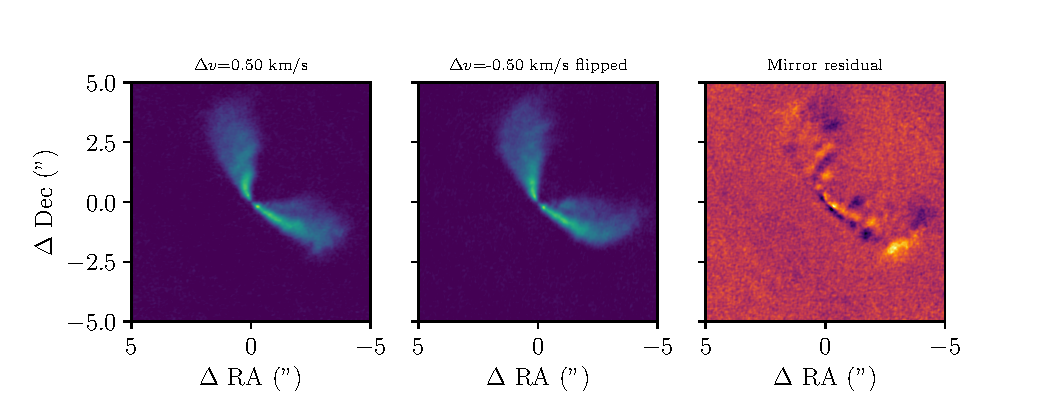
\includegraphics[width = 0.999\textwidth]{figures/channel060jvm.pdf}
    \caption{The left panel shows the $\Delta v = 0.5$ km/s velocity channel taken from the $0.15"$ resolution MAPS observations of HD~163296. The middle panel shows the corresponding $\Delta v = -0.5$ km/s interpolated from the cube. The right panel shows the residuals calculated by subtracting the middle image from the left image. We see that the bottom right velocity kink from \citet{calcino2022} shows up in the residuals as a bright blob.}
    \label{fig:mirror_residuals}
\end{figure}

Collapsing this cube along the velocity axis by taking for each pixel its value in the channel where it is brightest, the so-called peak intensity map or moment-8, yields a map of asymmetries in the disk.
This is shown in Figure~\ref{fig:mirror_M8}.
Two large bright arcs can be seen in the figure.
The bottom-most arc can be identified as the wake from the planet, which we demonstrate by plotting the wake shape projected to the emitting layer as in \citet{calcino2022}.
The other large bright arc does not seem to be associated with the planet wake, and has been previously identified by \citet{teague2021} and \citet{calcino2022}.

\begin{figure}
    \centering
    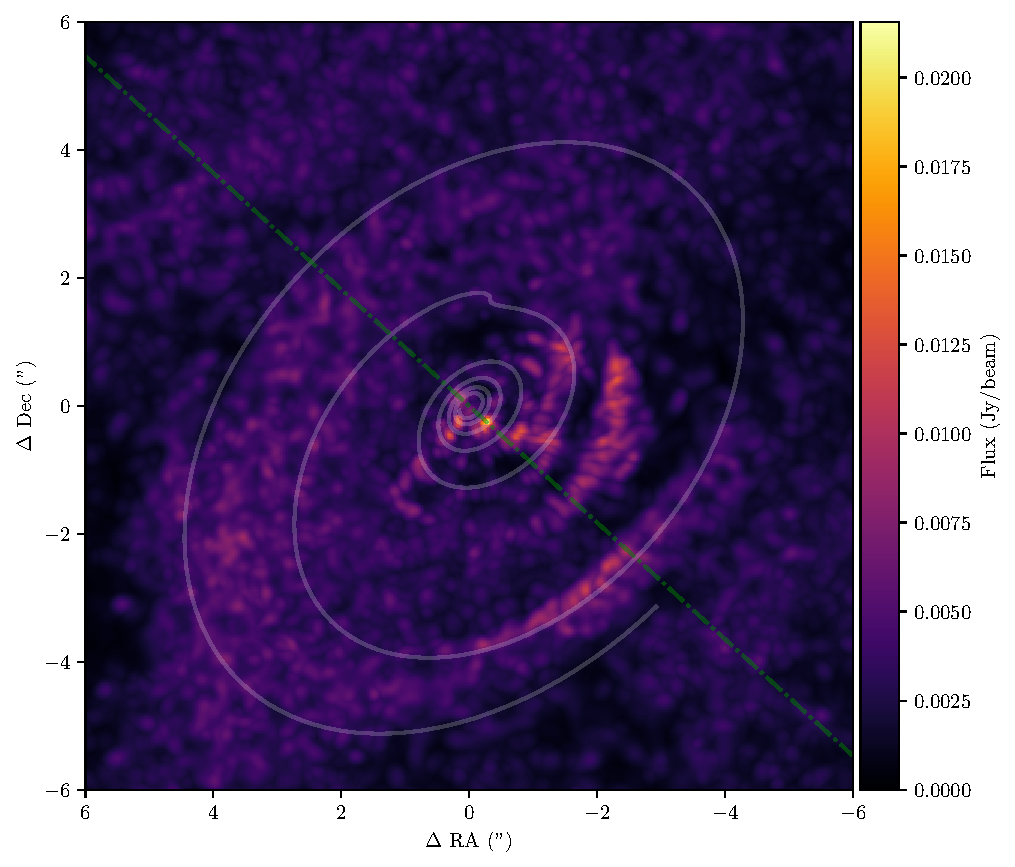
\includegraphics[width = 0.9\textwidth]{figures/mirror_M8.pdf}
    \caption{Peak intensity plot, generated from the mirror residuals of the MAPS $^{12}$CO kinematic observations of HD~163296 \citep{oberg2021}. Plotted also is the shape of the planet wake projected to the emitting layer from \citet{calcino2022}. We clearly see the planet wake as a bright arc in the bottom right of the image. Also identified is a further bright arc not associated with the planet wake, which has also been pointed out by \citet{teague2021} and \citet{calcino2022}. The green dot-dashed line shows the line of symmetry for the plot, since each half of the disk has been used to subtract the other half, it is ambiguous which side of the green line each feature in the map should actually be on.}
    \label{fig:mirror_M8}
\end{figure}

Extracting the perturbations associated with the wake in this way is valuable because unlike other methods \citep{teague2021,teague2022} it is completely model-independent.
It does however come with some important caveats, the first of which is a positional ambiguity in the features identified in the map shown in Figure~\ref{fig:mirror_M8}.
Since the residuals on each half of the disk are found by subtracting the other half, features that show up as positive residuals on one side of the disk will also show up as negative residuals on the other side.
One could obtain the symmetric partner of Figure~\ref{fig:mirror_M8} by taking instead the lowest intensity value in each channel from the mirror residuals cube.

Finally, it is not clear how this method may be used to extract velocity information, which is ultimately what we need to determine the planet mass.
We found that attempting to create a peak velocity map from the mirror residuals cube resulted in essentially just noise, and concluded that it is not very useful.
This is probably not surprising since the velocity of the channel where a particular pixel is brightest is not very meaningful for a pixel where there are no asymmetric features.


%\begin{itemize}
%    \item Describe method, makes use of symmetry
%    \item Present residuals 
%    \item Present peak intensity plot 
%    \item Present peak velocity plot
%    \item Discuss ambiguity
%    \item May be a promising way to make wakes more quantitatively
%    \item Hard to use to extract velocities
%\end{itemize}

%\section{Model-Independent Perturbation Extraction} \label{sec:isovelocity_transform}

%\begin{itemize}
%    \item Describe coordinate transform
%    \item Present example using analytics
%    \item Discuss its model dependence issue 
%    \item Describe how in principal this could be done independently of model, does not assume any background disk model, and does not assume axisymmetry of the disk
%    \item Should be able to extract only the planet perturbations
%\end{itemize}

